\chapter{Referencial Teórico}\label{referencial-teorico}

% ---
\section{Ciência Cidadã}
% ---

A Ciência Cidadã representa uma ponte entre a comunidade científica e o público geral, permitindo que pessoas sem formação científica formal possam contribuir em pesquisas científicas. Essa metodologia colaborativa tem se destacado em diversas áreas de pesquisa como na conservação da biodiversidade e na preservação ambiental. Através da Ciência Cidadã é possível que voluntários coletem e analisem dados, fornecendo informações que agregam no conhecimento acadêmico e auxiliam na resolução de questões sociais.

Segundo \citeonline{palma2016monitoramento}, trata-se de uma metodologia de pesquisa promissora na produção de conhecimento para ser aplicada em diversos campos científicos. Essa abordagem se destaca, em especial, com seu potencial de  geração de dados e análises, temporal e espacial, quando comparada com os métodos tradicionais de pesquisa. Para \citeonline{wildschut2017citizen}, a metodologia da ciência cidadã tem potencial para ampliar o escopo de pesquisas e aumentar e aprimorar a capacidade na coleta de dados e que os cidadãos que participam podem contribuir com informações importantes enquanto aprendem sobre as mais diversas áreas científicas.

A construção de conhecimento colaborativo realizado entre cidadãos e cientistas se mostra uma maneira poderosa de construção de conhecimentos, que agrega tanto no meio científico quanto social. Estes projetos instigam que as pessoas participem de maneira voluntária e ativa na resolução de situações do dia-a-dia da nossa sociedade, disseminando conhecimento de diversas áreas e fazendo com que diversos conteúdos saiam de suas bolhas científicas e obtenham um alcance maior.

% ---
\section{Agenda 2030}
% ---

A Agenda 2030 para o Desenvolvimento Sustentável é um plano de ação global adotado pelas Nações Unidas em 2015, com o objetivo de promover a prosperidade enquanto protege o planeta. Ela estabelece 17 Objetivos de Desenvolvimento Sustentável (ODS), que são subdivididos em 169 metas específicas. Esses objetivos englobam uma ampla gama de questões sociais, econômicas e ambientais, como erradicação da pobreza, igualdade de gênero, educação de qualidade, água limpa e saneamento, energia acessível e não poluente, trabalho decente e crescimento econômico \cite{onu2015ods}.

Segundo a organização, os ODS são projetados com os três pilares do desenvolvimento sustentável: econômico, social e ambiental. A Agenda enfatiza a importância de garantir que os direitos humanos de todos sejam realizados e que haja igualdade de gênero e empoderamento de mulheres e meninas. Além disso, reconhece que a erradicação da pobreza em todas as suas formas é o maior desafio global e, um requisito indispensável para o desenvolvimento sustentável.

A implementação da Agenda 2030 requer a mobilização de recursos e uma Parceria Global para o Desenvolvimento Sustentável, envolvendo todos os países, partes interessadas e pessoas. A Agenda é mundial, e se aplica a todos os países levando em conta diferentes realidades nacionais, capacidades e níveis de desenvolvimento. Ela promove a paz, justiça e instituições eficazes, e destaca a necessidade de ações urgentes sobre a mudança climática para proteger o planeta para as gerações presentes e futuras \cite{onu2015agenda2030}.

% ---
\section{Objetivos de Desenvolvimento Sustentável (ODS)}
% ---

Os ODS são um conjunto de 17 metas estabelecidas pelas Nações Unidas para abordar os principais desafios de desenvolvimento no Brasil e em todo o mundo. Esses objetivos visam criar um futuro mais justo, equitativo e sustentável para todos \cite{onu2015ods}. São eles:

\begin{itemize}
    \item \textbf{ODS 1}: Erradicação da Pobreza: Acabar com a pobreza em todas as suas formas, em todos os lugares.
    \item \textbf{ODS 2}: Fome Zero e Agricultura Sustentável: Garantir a segurança alimentar, melhorar a nutrição e promover a agricultura sustentável.
    \item \textbf{ODS 3}: Saúde e Bem-Estar: Assegurar uma vida saudável e promover o bem-estar para todas as idades.
    \item \textbf{ODS 4}: Educação de Qualidade: Garantir uma educação inclusiva, equitativa e de qualidade.
    \item \textbf{ODS 5}: Igualdade de Gênero: Alcançar a igualdade de gênero e empoderar todas as mulheres e meninas.
    \item \textbf{ODS 6}: Água Limpa e Saneamento: Garantir a disponibilidade e gestão sustentável da água e saneamento para todos.
    \item \textbf{ODS 7}: Energia Limpa e Acessível: Assegurar o acesso a fontes de energia acessíveis, confiáveis, sustentáveis e modernas.
    \item \textbf{ODS 8}: Trabalho Decente e Crescimento Econômico: Promover o crescimento econômico inclusivo e sustentável, emprego pleno e produtivo e trabalho decente para todos.
    \item \textbf{ODS 9}: Indústria, Inovação e Infraestrutura: Construir infraestruturas resilientes, promover a industrialização inclusiva e sustentável e fomentar a inovação.
    \item \textbf{ODS 10}: Redução das Desigualdades: Reduzir as desigualdades dentro e entre países.
    \item \textbf{ODS 11}: Cidades e Comunidades Sustentáveis: Tornar as cidades e os assentamentos humanos inclusivos, seguros, resilientes e sustentáveis.
    \item \textbf{ODS 12}: Consumo e Produção Responsáveis: Assegurar padrões de consumo e produção sustentáveis.
    \item \textbf{ODS 13}: Ação Contra a Mudança Global do Clima: Tomar medidas urgentes para combater a mudança climática e seus impactos.
    \item \textbf{ODS 14}: Vida na Água: Conservar e usar de forma sustentável os oceanos, mares e recursos marinhos.
    \item \textbf{ODS 15}: Vida Terrestre: Proteger, restaurar e promover o uso sustentável dos ecossistemas terrestres, gerir florestas de forma sustentável, combater a desertificação e deter a perda de biodiversidade.
    \item \textbf{ODS 16}: Paz, Justiça e Instituições Eficazes: Promover sociedades pacíficas e inclusivas para o desenvolvimento sustentável, proporcionar acesso à justiça para todos e construir instituições eficazes, responsáveis e inclusivas em todos os níveis.
    \item \textbf{ODS 17}: Parcerias e Meios de Implementação: Fortalecer os meios de implementação e revitalizar a parceria global para o desenvolvimento sustentável.
\end{itemize}

Os itens acima são um apelo global visando acabar com a pobreza, proteger o meio ambiente e o clima e garantir que as pessoas, em todos os lugares, possam desfrutar de paz e de prosperidade. São objetivos nos quais as Nações Unidas estão contribuindo para atingir a Agenda 2030 no Brasil \cite{onu2015ods}.

% ---
\section{Metodologia Iterativa Incremental}
% ---
A metodologia iterativa incremental é uma abordagem de desenvolvimento de \textit{software} que divide o processo em ciclos repetitivos. Cada iteração resulta em uma versão incrementada do \textit{software}, que é construída sobre a versão anterior com adições e melhorias. Segundo \citeonline{pressman2011engenharia}, essa metodologia permite que as equipes avaliem e integrem feedbacks mais rapidamente, adaptando-se às mudanças e refinando o produto ao longo do tempo. Isso contrasta com o modelo tradicional em cascata, onde cada fase deve ser concluída antes da próxima começar, sem retorno para fases anteriores.

De acordo com \citeonline{pressman2011engenharia}, o modelo incremental é uma abordagem de desenvolvimento de \textit{software} que foca na entrega gradual de funcionalidades em sucessivas versões incrementais. Nesse modelo, o desenvolvimento do \textit{software} é dividido em várias partes ou incrementos, cada um entregando uma versão operante do produto, que é aprimorada e expandida em lançamentos subsequentes.

\citeonline{pressman2011engenharia} afirma que o modelo incremental integra elementos de fluxos de processos lineares e paralelos. Na Figura~\ref{fig:incremental} é possível observar essa relação a partir das sequências lineares de forma escalonada que demonstram que ao longo do tempo cada incremento adiciona funcionalidades ou aprimoramentos ao sistema, permitindo uma evolução constante e contínua do produto final.

\begin{figure}[htb]
  \centering
  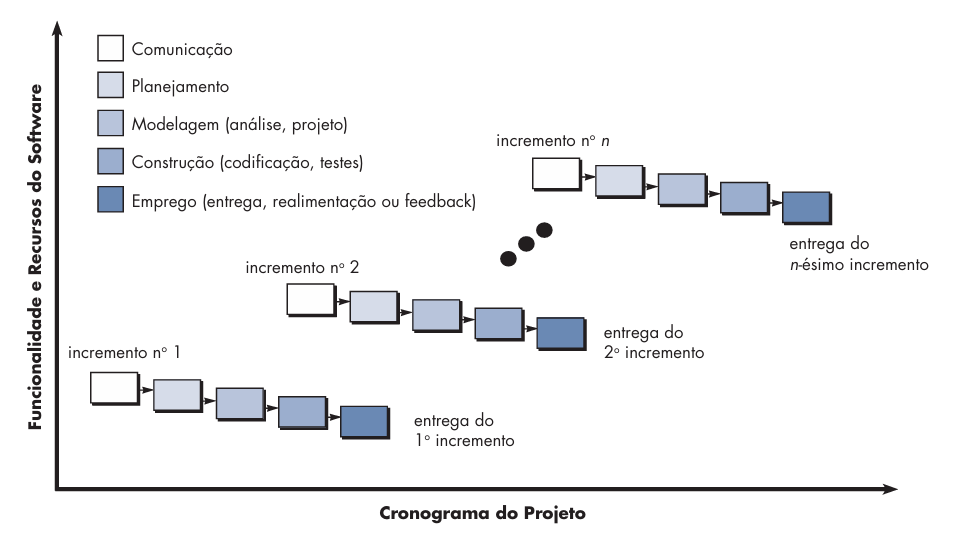
\includegraphics[width=0.8\textwidth]{imagens/graficoPressman.png}
  \caption{Ciclo de desenvolvimento incremental.}
  \legend{Fonte: \citeonline{pressman2011engenharia}.}
  \label{fig:incremental}
\end{figure}

% ---
\section{Kanban}
% ---

O Kanban é um método de gestão de fluxo de trabalho que fornece uma visualização 
das tarefas que devem ser realizadas, quando entregá-las e quanto ainda é necessário 
para finalizá-las com o objetivo de aumentar a eficiência e o entendimento do 
desenvolvimento \cite{ohno1988toyota}. Originou-se no sistema da Toyota no Japão 
dos anos 1940 e foi adaptado para o desenvolvimento de \textit{software} e sistemas de 
TI por David J. Anderson em 2004. Para isso, o Kanban utiliza de um quadro dividido em 
colunas para representar os diferentes estágios do trabalho, onde os cartões que 
representam as tarefas se movem de uma coluna para outra, refletindo o progresso real 
\cite{zayat2020framework}.

% ---
\section{Jira}
% ---

O \textit{Jira} é um \textit{software} comercial de gerenciamento de projetos desenvolvido 
pela empresa \citeonline{atlassian_jira_2025}. Ele permite a criação, acompanhamento e gerência de tarefas e projetos a partir de uma interface personalizável que suporta diversas metodologias ágeis como Scrum e Kanban, facilitando a colaboração e comunicação durante o desenvolvimento.

A ferramenta pode ser usada para planejar \textit{sprints}, atribuir tarefas, acompanhar 
\textit{bugs}, gerar relatórios e analisar o desempenho da equipe. Ele possui 
integração com uma variedade de ferramentas de desenvolvimento e oferece funcionalidades 
para personalizar fluxos de trabalho, campos e painéis, tornando-o adaptável às 
necessidades específicas de cada projeto ou organização.


\section{Tecnologias e Frameworks}\label{tecnologias}

Neste capítulo, serão apresentadas as tecnologias escolhidas para o 
desenvolvimento do aplicativo, destacando os aspectos que influenciaram nas 
escolhas e como elas contribuíram para o desenvolvimento do projeto.

\subsection{Flutter}

O \textit{Flutter} é um conjunto de ferramentas de UI (Interface do Usuário) criado 
pelo \textit{Google} em 2017. Se diferencia por possuir um suporte multiplataforma de código aberto 
projetado para permitir a reutilização de código em diversos sistemas operacionais, como \textit{iOS}, 
\textit{Android}, \textit{web} e \textit{desktop}, enquanto possibilita que as aplicações interajam 
diretamente com os serviços de cada plataforma. Como publicado por seus desenvolvedores, 
o \textit{Flutter} oferece 
uma solução centralizada para o desenvolvimento multiplataforma que facilita a criação de 
componentes visuais ao mesmo tempo em que realiza a integração com recursos nativos de cada tipo 
de dispositivo \cite{flutterDocs2025}.

Com esse \textit{framework}, os aplicativos são compilados a partir de um único código-base para as 
plataformas \textit{mobile}, \textit{web} e \textit{desktop}. O desenvolvimento no \textit{Flutter} é baseado em \textit{Widgets}, 
componentes escritos em \textit{Dart} que são responsáveis pela visualização das telas e pela interação 
com o usuário.
Esses componentes podem ou não estar associados a um estado, quando estão, são chamados de \textit{Stateful} 
\textit{Widgets} e, quando não, de \textit{Stateless} \textit{Widgets} \cite{flutterDocs2025}.

Além disso, o \textit{Flutter} possui a funcionalidade de \textit{hot reload}. 
Uma ferramenta que permite que alterações sejam feitas no código 
enquanto a aplicação está em execução, gerando uma 
atualização em tempo real da interface do usuário e da lógica da aplicação, 
mantendo inalterado seu estado de execução.

A escolha pelo \textit{Flutter} (versão 3.29.2) se deu principalmente pela sua capacidade multiplataforma a partir de 
uma única base de código, otimizando tempo e recursos. Outro fator decisivo foi a 
facilidade de integração com os diversos serviços do \textit{Firebase}, 
que facilitam a implementação de funcionalidades essenciais,  
como a autenticação, o banco de dados em tempo real e o armazenamento.

\subsection{Dart}

\textit{Dart} é uma linguagem de programação lançada pelo \textit{Google} em 2013, criada com foco em produtividade e 
performance para aplicações multiplataforma. A linguagem é orientada a objetos e oferece tipagem 
estática forte, porém também é possível optar pelo uso de tipagem dinâmica, 
o que pode ser útil em algumas situações. \cite{dartDocs2025}.

Um aspecto importante do \textit{Dart} é sua flexibilidade de compilação. 
É uma linguagem que utiliza tanto a compilação \textit{just-in-time} 
(JIT) quanto \textit{ahead-of-time} (AOT). 
Em tempo de desenvolvimento, o \textit{Dart} roda no \textit{Dart} VM 
usando JIT, o que permite recompilar apenas partes 
do código em tempo real sem reiniciar toda a aplicação. Essa funcionalidade 
viabiliza o recurso de \textit{hot reload} do \textit{Flutter}, permitindo 
que alterações sejam refletidas imediatamente na aplicação sem alterar o 
estado da interface.
Após realizar o lançamento de uma versão, o \textit{Dart} usa AOT para compilar o código diretamente 
para código nativo, o que garante um desempenho maior com relação ao JIT \cite{dartDocs2025}.

A escolha do Dart (versão 3.7.2) como linguagem de programação para o projeto se deu pela sua
proximidade com o \textit{Flutter}, pela tipagem forte, pelas características de 
programação orientada a objetos e pela facilidade de integração com o \textit{Firebase}.

\subsection{Firebase}

O \textit{Firebase} é uma plataforma de desenvolvimento de aplicativos móveis e \textit{web} 
fornecida pelo \textit{Google}, que oferece uma ampla gama de serviços \textit{backend} para 
facilitar a criação de aplicações robustas e escaláveis. Tem como característica 
permitir o desenvolvimento centralizado sem a necessidade de infraestrutura própria, 
fornecendo soluções completas para autenticação de usuários, banco de dados em tempo real, 
armazenamento de arquivos, envio de notificações, análises de uso e monitoramento de 
desempenho. Além disso, a plataforma integra ferramentas para teste, distribuição 
e acompanhamento do ciclo de vida do aplicativo com suporte multiplataforma \cite{firebase2025}.

Dentre os principais serviços disponibilizados no plano \textit{Spark} que foram 
utilizados no projeto, estão o \textit{Firebase Authentication}, 
que possibilita a autenticação de usuários via e-mail/senha e \textit{Google}, com suporte 
para até 50 mil usuários ativos mensais sem custo. O \textit{Firebase Analytics} que fornece 
relatórios detalhados sobre o comportamento e uso do aplicativo, permitindo a 
análise de métricas essenciais. O \textit{App Distribution} que possibilita a distribuição de versões 
de teste do aplicativo para usuários selecionados durante as fases de desenvolvimento e teste. 
Além do \textit{Cloud Firestore Database} que oferece até 1 GB de armazenamento, com limites diários de 50 
mil leituras, 20 mil gravações e 20 mil exclusões de documentos. E do \textit{Cloud Storage} que
disponibiliza 5 GB de armazenamento, 1 GB de download diário, além de 20 mil operações 
de upload e 50 mil operações de download por dia \cite{firebase2025}.

Neste projeto, o \textit{Firebase} foi escolhido para gerenciar a autenticação e o armazenamento de 
dados, utilizando o \textit{Firebase Authentication} para autenticar usuários com diferentes métodos de login e 
o \textit{Firebase Storage} para armazenar imagens, além do banco de dados NoSQL 
\textit{Cloud Firestore Database} para salvar os dados gerais do sistema e do Analytics para 
geração de \textit{dashboards} visando analisar o funcionamento geral da aplicação.
A definição pelo \textit{Firebase} se deu pela robustez e facilidade de integração com \textit{Flutter} 
oferecendo uma plataforma de backend eficiente e escalável. A aplicação foi construída com a 
utilização dos benefícios do plano \textit{Spark} descritos acima,
que, apesar de ser um plano gratuito, traz diversas ferramentas com limites de uso suficientemente 
altos para projetos iniciais.

\subsection{Pacotes e Plugins do Flutter}

Como o \textit{Flutter} possui uma arquitetura baseada em pacotes e \textit{plugins}, para o desenvolvimento 
de algumas funcionalidades específicas da aplicação proposta neste trabalho foram selecionados 
algumas dependências externas para facilitar e aumentar as possibilidades de desenvolvimento.

As dependências do projeto podem ser classificadas em três categorias. Bibliotecas puramente em Dart, 
que não interagem com \textit{APIs} nativas da 
plataforma, como \texttt{excel} (para manipulação de planilhas), \texttt{intl} (internacionalização 
e formatação de dados) e \texttt{diacritic} (remoção de acentos e caracteres especiais).

Plugins, que integram o código \textit{Dart} com \textit{APIs} nativas dos 
sistemas operacionais \textit{Android} e \textit{iOS}. Exemplos incluem \texttt{geolocator}
 (geolocalização), 
\texttt{image\_picker} (acesso à câmera e galeria) e \texttt{permission\_handler} (gerenciamento 
de permissões).

E as ferramentas auxiliares, que contribuem com a geração 
de código e automação de processos durante o desenvolvimento, como \texttt{hive\_generator} 
(geração de adaptadores para o \textit{Hive}) e \texttt{build\_runner} (execução de processos automáticos de 
geração de código).

Essas dependencias permitem incorporar funcionalidades reutilizáveis no projeto 
como renderização de mapas, autenticação com Firebase e diversos formatos de gráficos 
sem a necessidade de implementações manuais que seriam custosas e extensas. 
Além disso, possibilitam o acesso a recursos nativos dos dispositivo, como a 
geolocalização, gerenciamento de permissões, câmera e o armazenamento local no dispositivo.

A Tabela~\ref{tab:dependencias_flutter} apresenta todas as dependências utilizadas 
no projeto, especificando a versão de cada uma, bem como uma breve 
descrição de sua finalidade. Essa relação visa demonstrar a amplitude de recursos externos 
incorporados ao aplicativo e documentar as versões exatas para fins de controle de compatibilidade.

\begin{table}[H]
    \centering
    \caption{Dependências do Projeto \textit{Flutter}}
    \begin{tabular}{|p{4cm}|p{2.5cm}|p{8cm}|}
    \hline
    \textbf{Dependência} & \textbf{Versão} & \textbf{Descrição breve} \\ \hline
    flutter & sdk: flutter & Framework principal para desenvolvimento de apps móveis. \\ \hline
    flutter\_localizations & sdk: flutter & Suporte a localização (i18n) para Flutter. \\ \hline
    cupertino\_icons & \^{}1.0.2 & Ícones estilo iOS para Flutter. \\ \hline
    firebase\_core & \^{}3.8.1 & Inicialização e integração do Firebase. \\ \hline
    firebase\_auth & \^{}5.3.4 & Autenticação com Firebase. \\ \hline
    cloud\_firestore & \^{}5.4.4 & Integração com o banco Firestore. \\ \hline
    firebase\_analytics & \^{}11.3.3 & Monitoramento e análise de uso (analytics). \\ \hline
    firebase\_app\_check & \^{}0.3.2+5 & Segurança para apps usando Firebase. \\ \hline
    google\_sign\_in & \^{}6.2.2 & Autenticação via Google. \\ \hline
    persistent\_bottom\_nav\_bar & \^{}6.2.1 & Barra de navegação inferior persistente. \\ \hline
    image\_picker & \^{}1.1.2 & Seleção de imagens da galeria ou câmera. \\ \hline
    firebase\_storage & \^{}12.3.4 & Armazenamento de arquivos no Firebase. \\ \hline
    diacritic & \^{}0.1.3 & Remoção de acentos (diacríticos) de strings. \\ \hline
    provider & \^{}6.1.2 & Gerenciamento de estado simplificado. \\ \hline
    photo\_view & \^{}0.15.0 & Visualização de imagens com zoom e rotação. \\ \hline
    geolocator & \^{}13.0.2 & Geolocalização e rastreamento de posição. \\ \hline
    geocoding & \^{}3.0.0 & Geocodificação e reversa. \\ \hline
    phosphor\_flutter & \^{}2.1.0 & Ícones customizados da biblioteca Phosphor. \\ \hline
    url\_launcher & \^{}6.3.1 & Abertura de URLs externas (navegadores, apps, etc.). \\ \hline
    accordion & \^{}2.6.0 & Componente de interface tipo acordeão. \\ \hline
    cached\_network\_image & \^{}3.4.1 & Cache para imagens carregadas da web. \\ \hline
    hive & \^{}2.2.3 & Banco de dados local rápido e leve. \\ \hline
    hive\_generator & \^{}2.0.1 & Gerador de código para Hive. \\ \hline
    path\_provider & \^{}2.1.1 & Acesso a diretórios do sistema de arquivos. \\ \hline
    connectivity\_plus & \^{}5.0.2 & Detecção de status de conectividade (online/offline). \\ \hline
    build\_runner & \^{}2.4.8 & Utilitário para geração de código automático. \\ \hline
    skeletonizer & \^{}1.4.2 & Animação skeleton loader (placeholders enquanto carrega). \\ \hline
    badges & \^{}3.1.2 & Criação de badges/insígnias visuais. \\ \hline
    pie\_chart & \^{}5.4.0 & Gráficos de pizza. \\ \hline
    graphic & \^{}2.5.0 & Biblioteca de gráficos avançados. \\ \hline
    share\_plus & \^{}10.1.4 & Compartilhamento nativo de conteúdo. \\ \hline
    exif & \^{}3.0.1 & Leitura de dados EXIF de imagens. \\ \hline
    latlong2 & \^{}0.9.0 & Tipos de dados para latitude e longitude. \\ \hline
    open\_filex & \^{}4.3.4 & Abertura de arquivos em apps externos. \\ \hline
    excel & \^{}4.0.6 & Manipulação de arquivos Excel (.xlsx). \\ \hline
    flutter\_map & \^{}8.1.1 & Renderização de mapas (como o OpenStreetMap). \\ \hline
    intl & \^{}0.19.0 & Internacionalização e formatação de datas/números. \\ \hline
    permission\_handler & \^{}12.0.0+1 & Gerenciamento de permissões do sistema operacional. \\ \hline
    device\_info\_plus & \^{}11.3.3 & Informações detalhadas sobre o dispositivo. \\ \hline
    \end{tabular}
    \label{tab:dependencias_flutter}
    \legend{Fonte: Autor}
\end{table}
    
\subsubsection{Hive}

O Hive é um banco de dados leve e extremamente rápido, escrito inteiramente 
em \textit{Dart}, projetado para ser usado em aplicações Flutter e 
\textit{Dart} nativas. Ele segue o modelo de banco de dados chave-valor, 
oferecendo uma alternativa eficiente ao SQLite e a outros bancos de dados 
mais complexos, especialmente em contextos mobile \cite{hive2025}.

Nesse projeto, o Hive foi escolhido como opção de banco de dados local para armazenamento dos registros em momentos em que o dispositivo está offline, 
permitindo que até 40 registros sejam armazenados localmente e sincronizados assim que a conexão com a internet retornar.
A principal vantagem do Hive é a simplicidade e velocidade em dispositivos móveis.

\subsubsection{Flutter Map}
O \textit{Flutter Map} é um plugin gratuito, multiplataforma e de código aberto
que permite a renderização de mapas 
dentro de aplicativos \textit{Flutter}. Oferece uma interface fácil de usar 
para adicionar camadas, marcadores personalizados e interações em mapas.
Possui suporte de diversos provedores de mapas, como
\textit{OpenStreetMap}, \textit{Mapbox} e \textit{Google Maps}, 
permitindo que os desenvolvedores 
 escolham a fonte de dados que melhor atende às suas necessidades. 
 Além disso, ele oferece suporte a recursos avançados, como 
 geolocalização, desenho de rotas e manipulação de gestos do 
 usuário, adição de \textit{layers} \cite{flutter_map_doc}.
 
 Neste projeto, o \textit{Flutter Map} foi utilizado para renderizar o mapa
 com marcadores personalizados das localizações dos registros realizados 
 pelos usuários, permitindo uma visão geográfica dos dados coletados.

\subsubsection{Excel}

O \textit{excel} é uma biblioteca de código aberto para o
\textit{Dart} que permite a leitura e escrita de arquivos do Microsoft Excel 
no formato \textit{XLSX} com customizações avançadas de template \cite{excel_flutter}.
Neste projeto foi utilizada para construir a planilha de registros personalizada para download e compartilhamento.

\subsubsection{Graphic}

\textit{Graphic} é uma biblioteca de visualização de dados para \textit{Flutter}, 
baseada 
na Gramática de Gráficos de Leland Wilkinson. Com ela é possível criar gráficos 
personalizados de diversos tipos. Além disso, oferece suporte 
a interações avançadas como: seleção, legenda, tooltips, zoom, e animações 
para transições e carregamento dos gráficos \cite{graphic_flutter}.

A aplicação desta biblioteca no projeto foi pensada para gerar uma 
visualização gráfica dos dados de registos coletados para maior síntese de
algumas informações chaves.
Para o resultado final, foram gerados gráficos nos formatos de pizza e barras.
